\documentclass[12pt]{article}
\usepackage[english]{babel} 
\usepackage{fontspec}
\setmainfont{Free Sans}
\usepackage{fancyhdr}
\usepackage{xcolor}

% AMS math et autre
\usepackage{amsmath}
\usepackage{amsfonts}
\usepackage{amssymb}
\usepackage{xspace}
\usepackage{upgreek}

\graphicspath{{imgs/}}
\sloppy{}

\title{Mathematical model of pual leg epithelium}

\author{G. Gay}

\date{}

\begin{document}

\section{Architecture}


\subsection{The elementary cell}

The architecture of the epithelium model consists in a graph containing
\begin{itemize}
\item two types of vertices:
  \begin{itemize}
  \item The cell centres
  \item The appical junctions vertices
  \end{itemize}
\item and two types of edges:
  \begin{itemize}
  \item The junction edges, structuring the apical surface of the
    epithelium
  \item The cell to junction edges linking one cell to its
    neighbouring junction vertices.
  \end{itemize}
\end{itemize}

\begin{figure}[htbp]
  \centering
  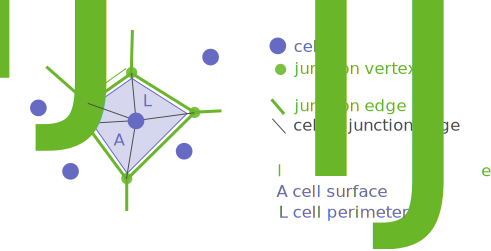
\includegraphics[width=6cm]{one_cell}
  \caption{A single cell in the epithelium, with its constituants}
  \label{fig:single_cell}
\end{figure}

\subsection{3D geometry}

The position of the vertices is given in two 3D coordinate systems,
Cartesian $(x, y, z)$ and cylindrical $(\rho, \theta, z)$.

Initially, the vertices are distributed over a cylinder centered around
the $z$ axis. The volume of a cell is computed as the sum of the area
of each triangle formed by a junction edge and two cell-to-junction
edges times the height of the cell center. Of course this is an
approximation:
$$
V_\alpha = \sum_{i,j} A_{\alpha ij} h_\alpha c_{\alpha i} c_{\alpha j} c_{ij}
$$
with $c_{uv} = 1$ if vertices $u$ and $v$ are connected and 0 otherwise.  
and $A_{\alpha ij} = || \mathbf{r}_{\alpha i} \times \mathbf{ r}_{\alpha j} || / 2 $



\end{document}




%%% Local Variables: 
%%% ispell-local-dictionary: "british"
%%% mode: latex
%%% TeX-master: t
%%% End: 
